\documentclass[a4paper,11pt]{article}
\usepackage[utf8]{inputenc}
\usepackage{graphicx}
\usepackage{enumerate}
\usepackage{geometry}
\usepackage{fancyhdr}
\usepackage{minted}
\usepackage{xcolor}
\usepackage{listings}
\usepackage[colorlinks = true,
            linkcolor = blue,
            urlcolor  = blue,
            citecolor = blue]{hyperref}

\geometry{total={210mm,297mm},
left=25mm,right=25mm,%
bindingoffset=0mm, top=20mm,bottom=20mm}

\graphicspath{ {./images/} }
\renewcommand{\thesubsubsection}{\thesubsection.\alph{subsubsection}}
\renewcommand*\sfdefault{phv}
\renewcommand\familydefault{\sfdefault}

% \renewcommand{\thesubsubsection}{\thesubsection.\alph{subsubsection}}

% \newmintedfile{html}{
%     linenos,
%     breaklines,
%     python3,
%     numbersep=8pt,
%     frame=single,
%     framesep=3mm} 

\newcommand*{\TitleFont}{%
      \usefont{\encodingdefault}{\rmdefault}{b}{n}%
      \fontsize{16}{20}%
      \selectfont}

\linespread{1.3}

% my own titles
\makeatletter
\renewcommand{\maketitle}{
\begin{center}
\vspace{2ex}
{\huge \textsc{\@title}}
\vspace{1ex}
\\
\rule{\linewidth}{0.5pt}\\
\@author \hfill \@date
\vspace{4ex}
\end{center}
}
\makeatother

\definecolor{bg}{rgb}{0.95,0.95,0.95}


% custom footers and headers
\pagestyle{fancy}
\lhead{}
\chead{}
\rhead{}
\lfoot{Assignment 8 : Web Servers }
\cfoot{}
\rfoot{Page \thepage}
\renewcommand{\headrulewidth}{0pt}
\renewcommand{\footrulewidth}{0pt}
%%----------%%%----------%%%----------%%%----------%%%

\begin{document}

\newminted{bash}{fontsize=\scriptsize, 
    linenos,
    breaklines,
    python3,
    numbersep=8pt,
    frame=single,
    bgcolor=bg,
    framesep=3mm} 

\newminted{python}{fontsize=\scriptsize, 
    linenos,
    breaklines,
    python3,
    numbersep=8pt,
    frame=single,
    bgcolor=bg,
    framesep=3mm} 

\newminted{html}{fontsize=\scriptsize, 
    linenos,
    breaklines,
    python3,
    numbersep=8pt,
    frame=single,
    bgcolor=bg,
    framesep=3mm}

\newminted{nginx}{fontsize=\scriptsize, 
    linenos,
    breaklines,
    python3,
    numbersep=8pt,
    frame=single,
    bgcolor=bg,
    framesep=3mm} 

% \newminted{all}{linenos, frame=single}

% \usemintedstyle{monokai}
\usemintedstyle{manni}
% \usemintedstyle{xcode}
% \usemintedstyle{vs}
% \usemintedstyle{autumn}
% \usemintedstyle{colorful}
% \usemintedstyle{trac}


\title{ \TitleFont Assignment 8 : Web Servers }

\author{Emil Sharifulllin, Innopolis University}

\date{\today}

\maketitle
\tableofcontents

\section{History}
\subsection{Can you think of reasons for the change in popularity of Apache? Explain.}
When nginx created apache worked only in mpm\_prefork which means that apache creates new process on every request this approach decrease performance on static requests and needs a lot of resources serve high load site. Also apache couldn't solve 10k problem when nginx created.

\section{Installation}
\addtocounter{subsection}{1}
\subsection{Older source trees like Apache 2.2.*, and nginx 1.6.* are still maintained. Can you think of reasons why?}
Old versions of web servers are still maintained because there is a lot of sites that uses old versions and if maintaining will end this sites will be vulnerable for new exploits.\\\\
My table number is 10 so I need to install nginx as a web server. Here is described steps to install nginx.
\begin{bashcode}
$ wget http://nginx.org/download/nginx-1.11.4.tar.gz
$ wget http://nginx.org/download/nginx-1.11.4.tar.gz.asc
$ gpg --recv-keys A1C052F8
$ gpg --verify nginx-1.11.4.tar.gz.asc
gpg: Good signature from "Maxim Dounin <mdounin@mdounin.ru>"
$ tar -xzvf nginx-1.11.4.tar.gz
$ ./configure --with-http_ssl_module --with-pcre --with-pcre-jit --with-http_v2_module --with-threads --with-http_stub_status_module
$ make
$ make install
$ ln -s /usr/local/nginx/sbin/nginx /usr/bin
\end{bashcode}
Nginx default installation folder is /usr/ocal/nginx so we don't need to set it manually.b
Nginx settins is stored in /usr/local/nginx/conf. To check configuration i used nginx -t

\begin{bashcode}
$ nginx -t
nginx: the configuration file /usr/local/nginx/conf/nginx.conf syntax is ok 
nginx: configuration file /usr/local/nginx/conf/nginx.conf test is successful
\end{bashcode}

\section{Virtual Hosts}
\addtocounter{subsection}{2}
\subsection{Implement virtual hosting in the web server for the virtual domains anyname.st[X].os3.su, anyname.st[X-1].os3.su and anyname.st[X+1].os3.su. Show your configuration.}
To implement virtual hosts I asked my neighbours to delegate me subdomains of their domains. Now I have two delegated domains: \href{http://st10.st9.os3.su}{st10.st9.os3.su} and \href{http://st10.st11.os3.su}{st10.st11.os3.su}. After DNS delegation I created two virual hosts in nginx.conf.

\begin{nginxcode*}{label=nginx.conf}
...
    server {
        listen  80;
        server_name     st10.st9.os3.su;
        location        / {
                root    /var/www/st9;
                index   index.html;
        }
    }

    server {
        listen  80;
        server_name     st10.st11.os3.su;
        location        / {
                root    /var/www/st11;
                index   index.html;
        }
    }
...
\end{nginxcode*}

\subsection{Create a simple, unique HTML page for each virtual host make sure that the server can correctly serve it. Please include virtualhost name to the main page.}

\begin{htmlcode*}{label=/var/www/st11/index.html}
<!DOCTYPE html>
<html>
<head>
  <title></title>
</head>
<body>
  Hello guest! This is st10.st11.os3.su
</body>
</html>
\end{htmlcode*}

\begin{htmlcode*}{label=/var/www/st9/index.html}
<!DOCTYPE html>
<html>
<head>
  <title></title>
</head>
<body>
  Hello guest! This is st10.st9.os3.su
</body>
</html>
\end{htmlcode*}


\subsection{Use curl to display the contents of a full HTTP/1.1 session served by your server. Explain the meaning of each request and reply header.
}

\begin{bashcode}
$ curl -v st10.st11.os3.su
* Rebuilt URL to: st10.st11.os3.su/
*   Trying 188.130.155.43...
* Connected to st10.st11.os3.su (188.130.155.43) port 80 (#0)
> GET / HTTP/1.1
> Host: st10.st11.os3.su
> User-Agent: curl/7.49.1
> Accept: */*
> 
< HTTP/1.1 200 OK
< Server: nginx/1.11.4
< Date: Thu, 06 Oct 2016 17:24:53 GMT
< Content-Type: text/html
< Content-Length: 117
< Last-Modified: Thu, 06 Oct 2016 12:58:00 GMT
< Connection: keep-alive
< ETag: "57f64a58-75"
< Accept-Ranges: bytes
< 
<!DOCTYPE html>
<html>
<head>
  <title></title>
</head>
<body>
  Hello guest! This is st10.st11.os3.su
</body>
</html>
* Connection #0 to host st10.st11.os3.su left intact
\end{bashcode}
This output means:\\
\textbf{Request}
\begin{itemize}
  \item The first line in HTTP/1.1 requires three things: HTTP method, path and protocol version delimited with spaces.
  \item From second line started headers and header "Host" is only one required by specification header. This header defines hostaname of server and is very useful for virtua; domains.
  \item Second header "User-Agent" is header that specifies software and system from which request started.
  \item "Accept" header defines certain media types which are acceptable for the response.
\end{itemize}
\textbf{Response}
\begin{itemize}
  \item First line of response is a special line whixh contains protocol version, response code and code definition.
  \item "server" header specifies type and version of web server that served this request.
  \item "Date" header inform client about datetime at server and this header often uses for caching of http responses.
  \item "Content-Type" tells to client what kind of content contains response.
  \item "Content-Length" used in client to understand how much data response contains.
  \item "Connection" header which set to "keep-alive" tells to client not to break connection after request.
  \item "Accept-Ranges" header allows the server to indicate its acceptance of range requests for a resource
  \item "ETag" response header field provides the current value of the entity tag for the requested variant
\end{itemize}

\section{Encryption}
\addtocounter{subsection}{5}
\subsection{Configure your web server to support TLS. Make sure you disable the SSLv2+3 and TLSv1.0+1.1 protocols as they are shown to be unsafe.}
To configure TLS I added this lines to nginx.conf.

\begin{nginxcode*}{label=nginx.conf}
server {
    listen  80;
    server_name     st10.os3.su;
    location        / {
            rewrite ^(.*)$ https://st10.os3.su$1 permanent;
    }
}
    server {
    listen       443 ssl http2;
    server_name  st10.os3.su;

    auth_basic           "closed site";
    auth_basic_user_file passwd.txt;

    ssl_certificate       /etc/certs/st10.os3.su.crt;
    ssl_certificate_key   /etc/certs/st10.os3.su.key;
    ssl_session_timeout  5m;
    ssl_session_cache   shared:SSL:10m;
    ssl_prefer_server_ciphers on;
    ssl_stapling on;
    resolver 8.8.8.8;
    add_header Strict-Transport-Security 'max-age=604800';

    ssl_ciphers  HIGH:!aNULL:!MD5;
    ssl_protocols TLSv1.2;
    ssl_prefer_server_ciphers  on;

    location / {
        root   /var/www/st10;
        index  index.html;
    }
}
\end{nginxcode*}
This configurations means:
\begin{itemize}
  \item \textbf{ssl\_session\_cache shared:SSL:10m; ssl\_session\_timeout 5m;} sets the timeout and type for caching. If client will send new request during ttl new handshake will not created.
  \item \textbf{ssl\_prefer\_server\_ciphers on;} Use server ciphers rather then client ciphers. Client ciphers may be vulnerable.
  \item \textbf{ssl\_stapling on;} Tells server to add signed OSCP headers to response.
  \item \textbf{ssl\_certificate and ssl\_certificate\_key} specifies certificate and key files.
  \item \textbf{add\_header Strict-Transport-Security 'max-age=604800';} not allow user to skip to insecure HTTP connection.
  \item \textbf{ssl\_protocols TLSv1.2;} allows use only TLS 1.2 because 1.0 and 1.1 are insecure.
  \item \textbf{ssl\_ciphers  HIGH:!aNULL:!MD5;} tells to server which ciphers to use.
\end{itemize}


\subsection{List the encryption standards / cipher suites that the web server supports with the standard configuration file. Select one and explain all its components.}
Nginx supports all ciphers that supported by openssl library. To get list of ciphers I ran command openssl ciphers.

\begin{itemize}
\item ECDHE-RSA-AES256-GCM-SHA384
\item ECDHE-ECDSA-AES256-GCM-SHA384
\item ECDHE-RSA-AES256-SHA384
\item ECDHE-ECDSA-AES256-SHA384
\item ECDHE-RSA-AES256-SHA
\item ECDHE-ECDSA-AES256-SHA
\item SRP-DSS-AES-256-CBC-SHA
\item SRP-RSA-AES-256-CBC-SHA
\item SRP-AES-256-CBC-SHA
\item DH-DSS-AES256-GCM-SHA384
\item DHE-DSS-AES256-GCM-SHA384
\item DH-RSA-AES256-GCM-SHA384
\item DHE-RSA-AES256-GCM-SHA384
\item DHE-RSA-AES256-SHA256
\item DHE-DSS-AES256-SHA256
\item DH-RSA-AES256-SHA256
\item DH-DSS-AES256-SHA256
\item DHE-RSA-AES256-SHA
\item DHE-DSS-AES256-SHA
\item DH-RSA-AES256-SHA
\item DH-DSS-AES256-SHA
\item DHE-RSA-CAMELLIA256-SHA
\item DHE-DSS-CAMELLIA256-SHA
\item DH-RSA-CAMELLIA256-SHA
\item DH-DSS-CAMELLIA256-SHA
\item ECDH-RSA-AES256-GCM-SHA384
\item ECDH-ECDSA-AES256-GCM-SHA384
\item ECDH-RSA-AES256-SHA384
\item ECDH-ECDSA-AES256-SHA384
\item ECDH-RSA-AES256-SHA
\item ECDH-ECDSA-AES256-SHA
\item AES256-GCM-SHA384
\item AES256-SHA256
\item AES256-SHA
\item CAMELLIA256-SHA
\item PSK-AES256-CBC-SHA
\item ECDHE-RSA-AES128-GCM-SHA256
\item ECDHE-ECDSA-AES128-GCM-SHA256
\item ECDHE-RSA-AES128-SHA256
\item ECDHE-ECDSA-AES128-SHA256
\item ECDHE-RSA-AES128-SHA
\item ECDHE-ECDSA-AES128-SHA
\item SRP-DSS-AES-128-CBC-SHA
\item SRP-RSA-AES-128-CBC-SHA
\item SRP-AES-128-CBC-SHA
\item DH-DSS-AES128-GCM-SHA256
\item DHE-DSS-AES128-GCM-SHA256
\item DH-RSA-AES128-GCM-SHA256
\item DHE-RSA-AES128-GCM-SHA256
\item DHE-RSA-AES128-SHA256
\item DHE-DSS-AES128-SHA256
\item DH-RSA-AES128-SHA256
\item DH-DSS-AES128-SHA256
\item DHE-RSA-AES128-SHA
\item DHE-DSS-AES128-SHA
\item DH-RSA-AES128-SHA
\item DH-DSS-AES128-SHA
\item DHE-RSA-SEED-SHA
\item DHE-DSS-SEED-SHA
\item DH-RSA-SEED-SHA
\item DH-DSS-SEED-SHA
\item DHE-RSA-CAMELLIA128-SHA
\item DHE-DSS-CAMELLIA128-SHA
\item DH-RSA-CAMELLIA128-SHA
\item DH-DSS-CAMELLIA128-SHA
\item ECDH-RSA-AES128-GCM-SHA256
\item ECDH-ECDSA-AES128-GCM-SHA256
\item ECDH-RSA-AES128-SHA256
\item ECDH-ECDSA-AES128-SHA256
\item ECDH-RSA-AES128-SHA
\item ECDH-ECDSA-AES128-SHA
\item AES128-GCM-SHA256
\item AES128-SHA256
\item AES128-SHA
\item SEED-SHA
\item CAMELLIA128-SHA
\item PSK-AES128-CBC-SHA
\item ECDHE-RSA-RC4-SHA
\item ECDHE-ECDSA-RC4-SHA
\item ECDH-RSA-RC4-SHA
\item ECDH-ECDSA-RC4-SHA
\item RC4-SHA
\item RC4-MD5
\item PSK-RC4-SHA
\item ECDHE-RSA-DES-CBC3-SHA
\item ECDHE-ECDSA-DES-CBC3-SHA
\item SRP-DSS-3DES-EDE-CBC-SHA
\item SRP-RSA-3DES-EDE-CBC-SHA
\item SRP-3DES-EDE-CBC-SHA
\item EDH-RSA-DES-CBC3-SHA
\item EDH-DSS-DES-CBC3-SHA
\item DH-RSA-DES-CBC3-SHA
\item DH-DSS-DES-CBC3-SHA
\item ECDH-RSA-DES-CBC3-SHA
\item ECDH-ECDSA-DES-CBC3-SHA
\item DES-CBC3-SHA
\item PSK-3DES-EDE-CBC-SHA
\end{itemize}

\subsection{Describe how you created your own certificate for your web server.}
I used certificate given for us by Azat. But you actually can create your own self-signed certificate with openssl library.

\subsection{You can test your secure web server using a web browser, but you can also use openssl and curl. Test your web server using both these tools, and report your findings.}

\begin{center}

\includegraphics[width=17cm]{browser}
\end{center}

\begin{bashcode}
$ curl -v https://st10.os3.su  
* Rebuilt URL to: https://st10.os3.su/
*   Trying 188.130.155.43...
* Connected to st10.os3.su (188.130.155.43) port 443 (#0)
* TLS 1.2 connection using TLS_ECDHE_RSA_WITH_AES_256_GCM_SHA384
\end{bashcode}

\subsection{Can you enable HTTPS for all your virtual hosts? Explain how you can configure one web server to serve multiple TLS enabled domains.}
With this certain certificate we cannot provide TLS security for all my virtual domains. This certificate can be used only with stX.os3.su domains. To enable HTTPS for other vortual domains I need to create wildcard certificate or create new certificate to every new domain.

\section{Web Server Security}
\addtocounter{subsection}{10}
\subsection{Investigate what configuration options there are on your assigned Web server that govern access rights. What ways are there to use these options on documents (folder access rights, IP acl, authentification methods, htaccess, robot.txt)?}
For better security it's necessary to set right permissions to root folders of websites. In my opinion for site root folder best permissions is: 755 for directories and 644 for files and owner www. The main purpose not to give execution rights to root foldes is that in some cases adversors can upload and execute scripts to this folder.\\
For IP ACL in nginx you can use allow and deny directives. This directives will tell server from which IP addresses allow requests.
\begin{nginxcode}
deny  192.168.1.1;
allow 192.168.1.0/24;
\end{nginxcode}
Nginx supports two kinds of authentication: basic HTTP authentication and JWT. I setted up basic auth.
\begin{bashcode}
$ openssl passwd qweasdzx
28.vsh2fqcrjU
\end{bashcode}

\begin{bashcode*}{label=passwd.txt}
litleleprikon:28.vsh2fqcrjU
\end{bashcode*}

\begin{nginxcode*}{label=nginx.conf}
auth_basic           "closed site";
auth_basic_user_file passwd.txt;
\end{nginxcode*}
File robots.txt tells to search engines which subdirectories of site to handle. With this file you can deny web crawlers to travel on some pieces of your site.


\subsection{Now create two web pages, one with asimple SSI instruction and one withasimple Perl/Python/Ruby CGI script (beware of Shellshock). Set up your web server so that only code on these pages can be executed (if possible).}

To add CGI I installed fastcgi package and added following lines to config file.
\begin{nginxcode*}{label=nginx.conf}
location /cgi-bin/ {
        fastcgi_pass unix:/var/run/fcgiwrap.socket;
        include fastcgi_params;
        fastcgi_param SCRIPT_FILENAME /var/www/st10/cgi.py;
}
\end{nginxcode*}

\begin{pythoncode*}{label=/var/www/st10/cgi.py}
#!/usr/bin/env python3
print("""HTTP/1.1 200 OK
Hello world"")
\end{pythoncode*}
To implement SSI I added ssi on; to nginx.conf and added file to root directory

\begin{htmlcode*}{label=/var/www/st10/ssi.html}
<html><body><h1><!--#echo var="DATE_LOCAL" --> </h1></body></html>
\end{htmlcode*}

\begin{center}
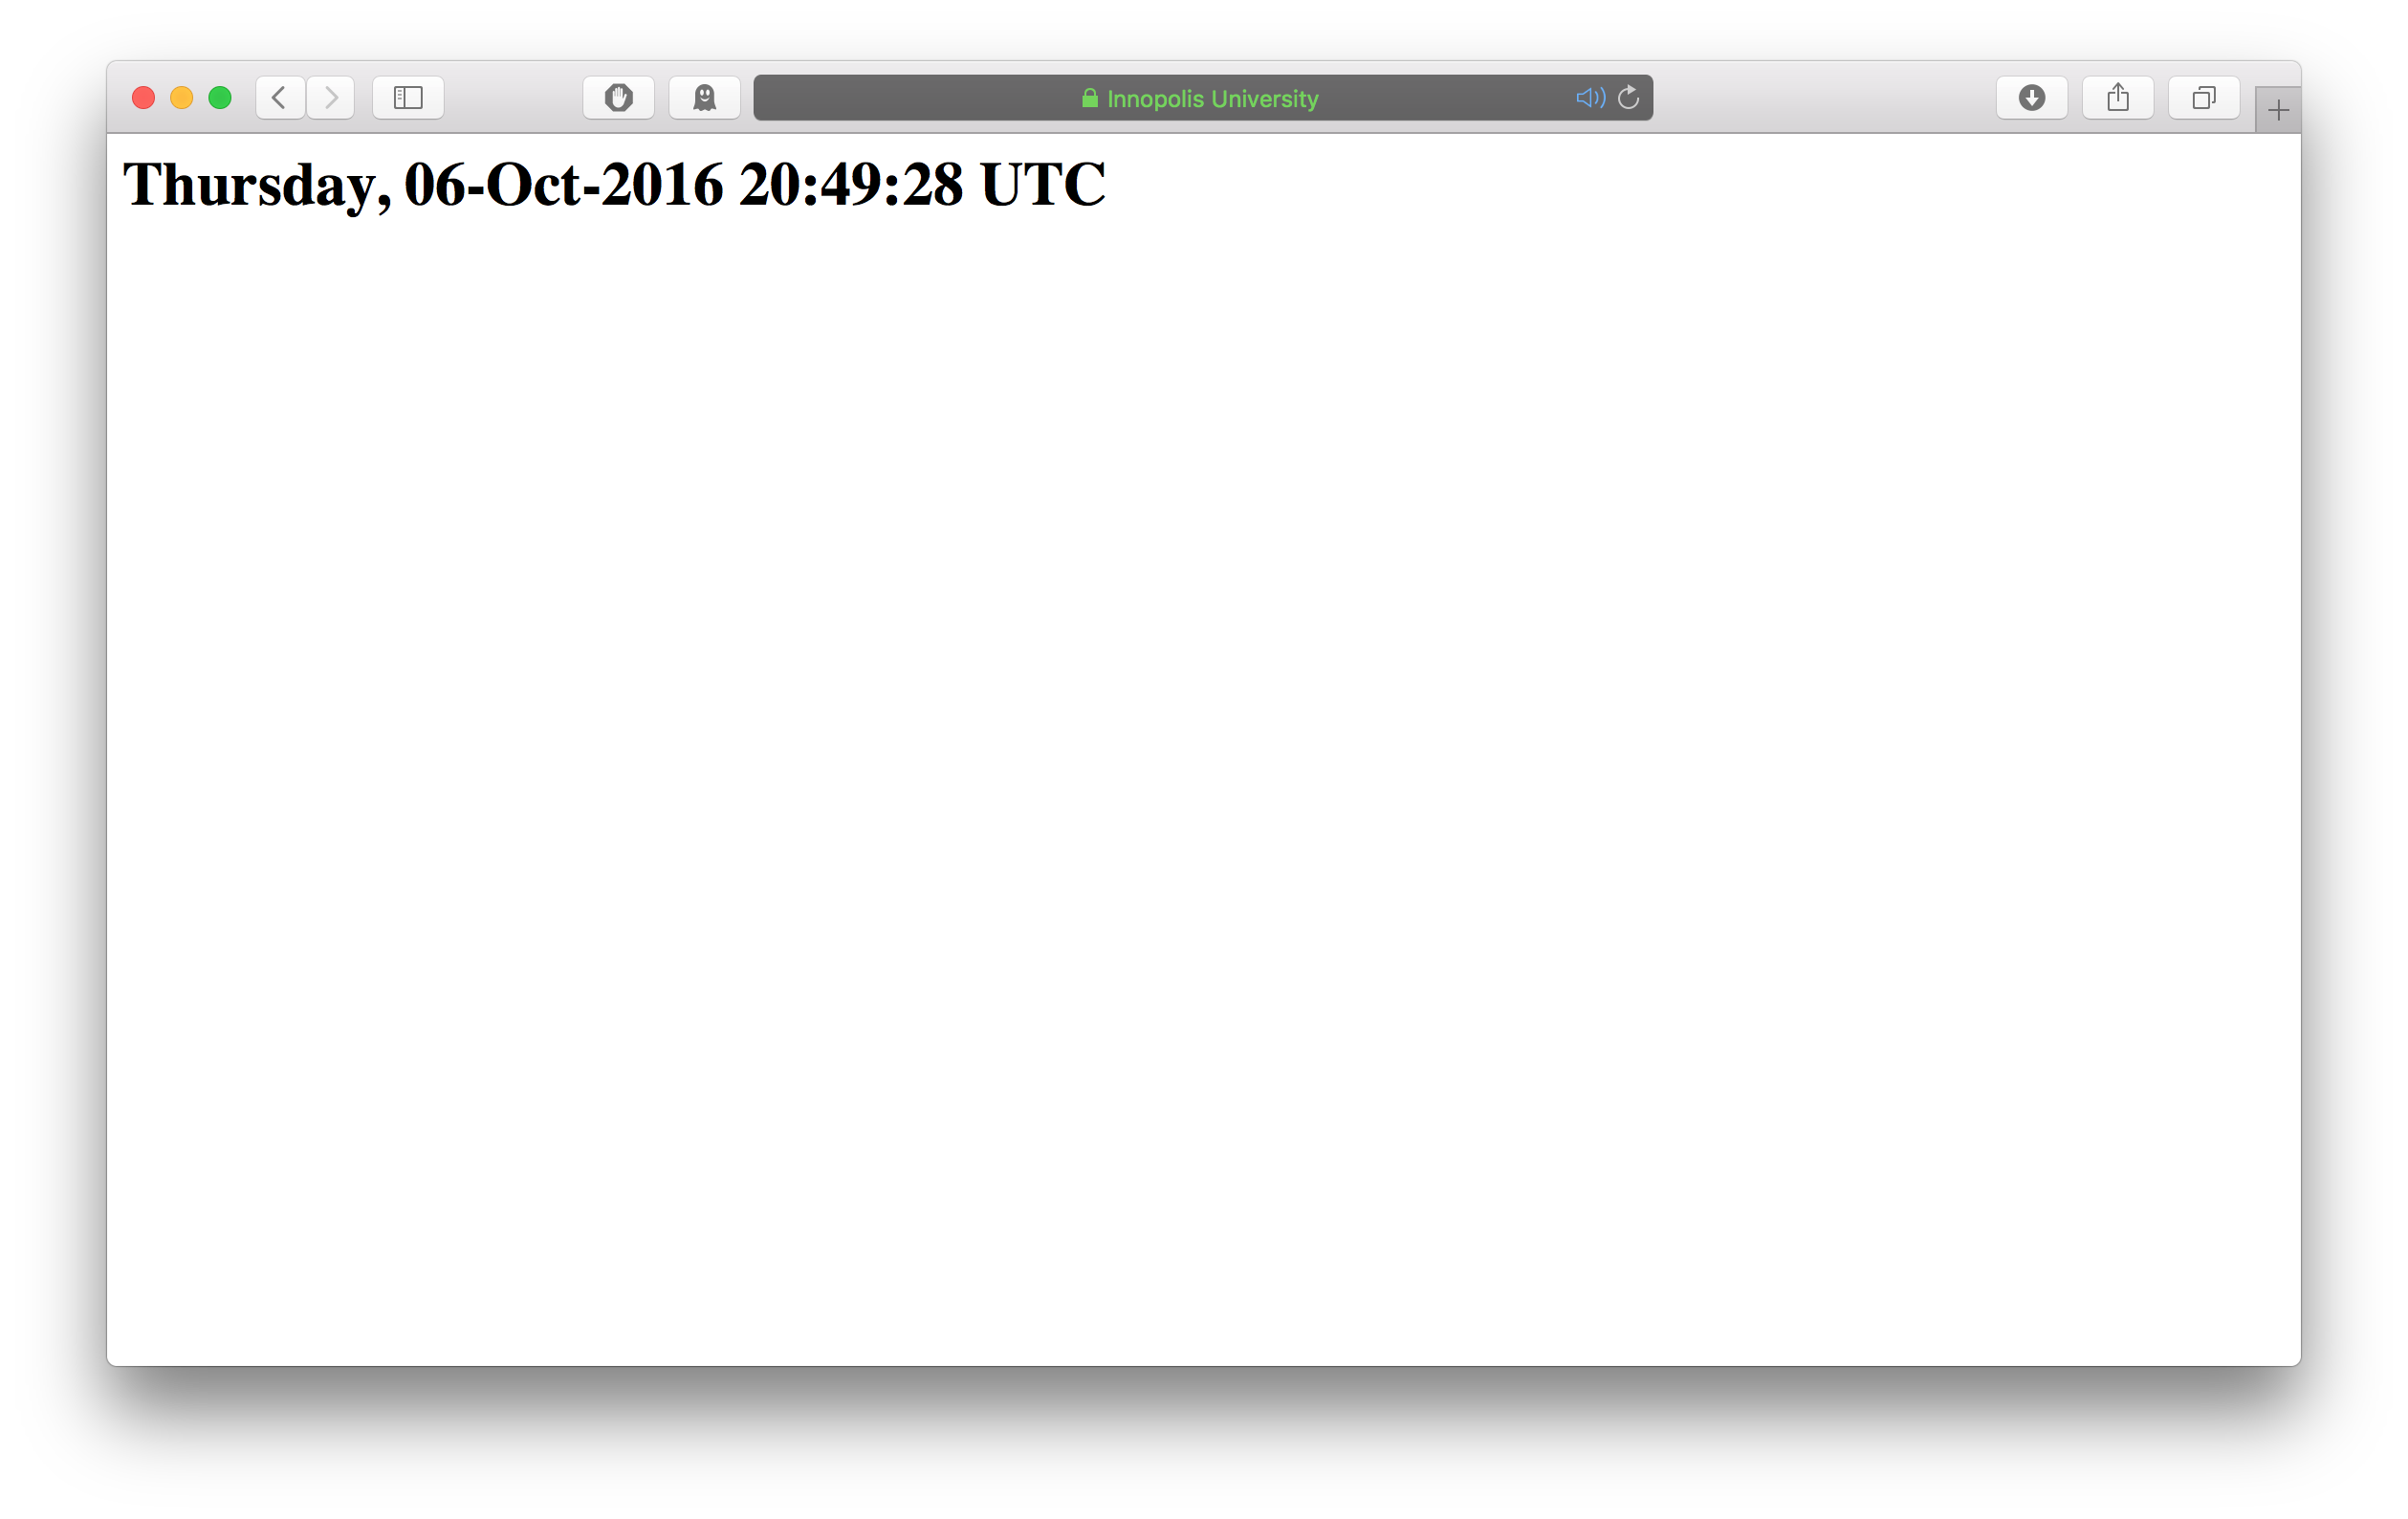
\includegraphics[width=17cm]{ssi}
\end{center}
\end{document}